\documentclass[12pt]{article}
\parindent=.25in

\setlength{\oddsidemargin}{0pt}
\setlength{\textwidth}{440pt}
\setlength{\topmargin}{0in}

\usepackage{amsmath}
\usepackage[dvips]{graphicx}
\usepackage{verbatim}
\usepackage{appendix}

\usepackage{amssymb}
\usepackage{amsfonts}
\usepackage{latexsym}
\usepackage[center]{subfigure}
\usepackage{epsfig}
\usepackage{hyperref}

\title{Stat 4201 Homework 8}
\author{Mengqi Zong $<mz2326@columbia.edu>$}

\begin{document}

\maketitle

% no paragraph indentation
\setlength{\parindent}{0in}

\section*{Question 1}

a) Here is the logistic regression of carrier on CK and H:

\begin{verbatim}
> summary(fit.p1)

Call:
glm(formula = Y ~ CK + H, family = binomial)

Deviance Residuals: 
     Min        1Q    Median        3Q       Max  
-2.44845  -0.38658  -0.19898   0.00193   2.44680  

Coefficients:
             Estimate Std. Error z value Pr(>|z|)    
(Intercept) -16.16597    3.65519  -4.423 9.75e-06 ***
CK            0.06838    0.01510   4.530 5.91e-06 ***
H             0.12731    0.03461   3.679 0.000234 ***
---
Signif. codes:  0 ‘***’ 0.001 ‘**’ 0.01 ‘*’ 0.05 ‘.’ 0.1 ‘ ’ 1 

(Dispersion parameter for binomial family taken to be 1)

    Null deviance: 149.840  on 119  degrees of freedom
Residual deviance:  62.224  on 117  degrees of freedom
AIC: 68.224

Number of Fisher Scoring iterations: 8
\end{verbatim}

Here is the confidence intervals:

\begin{verbatim}
> confint(fit.p1) 
Waiting for profiling to be done...
                   2.5 %     97.5 %
(Intercept) -24.48506599 -9.9576930
CK            0.04263730  0.1028274
H             0.06708505  0.2042785
There were 34 warnings (use warnings() to see them)
\end{verbatim}

I notice that using the H and CK will lead to the following
warning: 

\begin{verbatim}
fit.p1 <- glm(Y~CK+H, family=binomial)
Warning message:
glm.fit: fitted probabilities numerically 0 or 1 occurred 
\end{verbatim}

I find out that this indicates that some of the CK values are too
large to fit the model and CK needs a transformation. Since problem 2
explores about which predictor is appropriate, I just leave the
appropriate logitstic regression model to problem 2. \\

b) \\
$\beta_{CK}$: If $CK$ increases by 1 unit, the odds Y = 1 will
change by a multiplicative factor of $exp(\beta_{CK})$, other
variables being the same. \\

$\beta_H$: If $H$ increases by 1 unit, the odds Y = 1 will
change by a multiplicative factor of $exp(\beta_H)$, other
variables being the same. \\

\section*{Question 2}

a) The scatterplot of H versus log(CK) is shown in
Fig-\ref{fig:scatter}. As we can see, most of the squares in the plot
are in the district where log(CK) is low. As to H, there isn't such
concentration on the plot. So log(CK) might be useful predictors of
whether a woman is a carrier. \\

\begin{figure}[ht!]
  \centering
  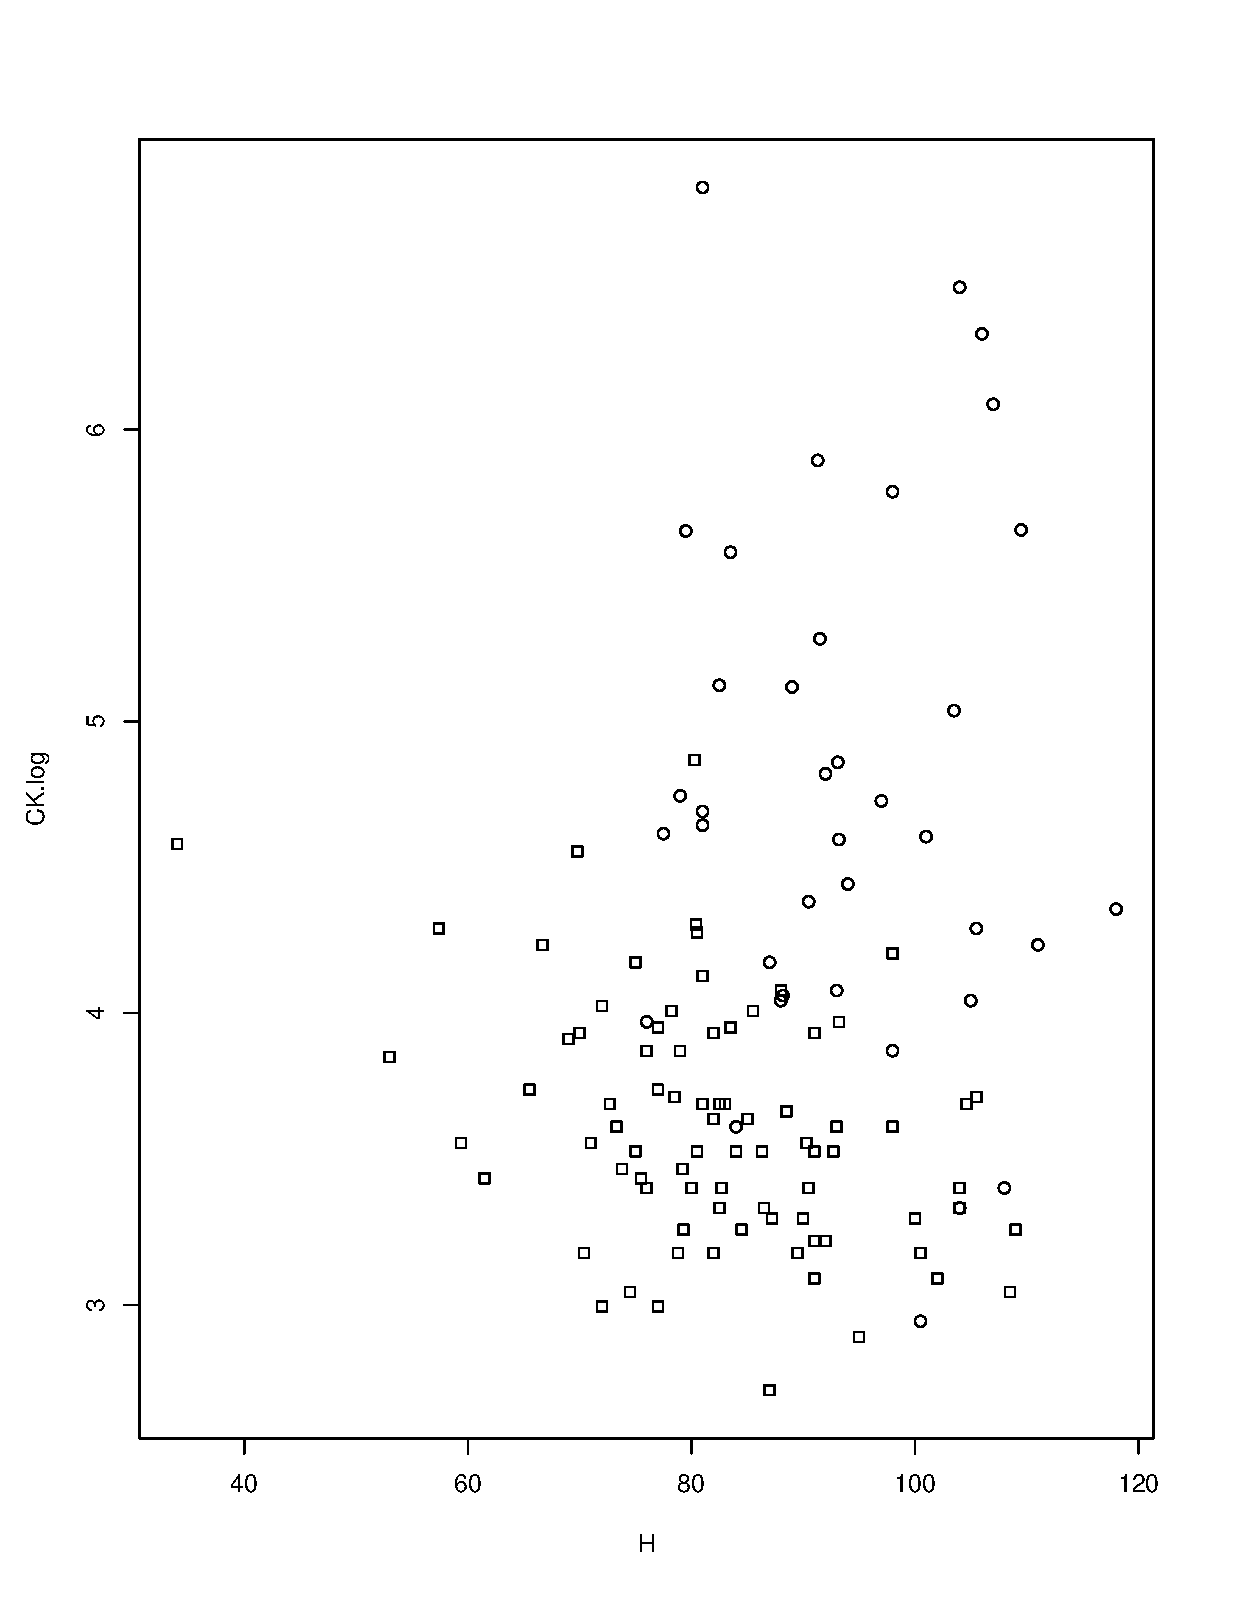
\includegraphics[width=0.7\textwidth]{scatter}
  \caption{Scatterplot: H versus log(CK) \label{fig:scatter}}
\end{figure}

b) \\
The logistic regression of carrier on CK and CK-squared:

\begin{verbatim}
> summary(fit.b1)

Call:
glm(formula = Y ~ CK + CK.square, family = binomial)

Deviance Residuals: 
     Min        1Q    Median        3Q       Max  
-2.27518  -0.51824  -0.37943   0.03892   2.50614  

Coefficients:
              Estimate Std. Error z value Pr(>|z|)    
(Intercept) -4.181e+00  7.272e-01  -5.749 8.96e-09 ***
CK           5.805e-02  1.301e-02   4.460 8.18e-06 ***
CK.square   -5.060e-05  3.286e-05  -1.540    0.124    
---
Signif. codes:  0 ‘***’ 0.001 ‘**’ 0.01 ‘*’ 0.05 ‘.’ 0.1 ‘ ’ 1 

(Dispersion parameter for binomial family taken to be 1)

    Null deviance: 149.840  on 119  degrees of freedom
Residual deviance:  85.435  on 117  degrees of freedom
AIC: 91.435

Number of Fisher Scoring iterations: 9
\end{verbatim}

As we can see, CK-squared term does not significantly differ from 0. \\

The logistic regression of carrier on log(CK) and $[log(CK)]^2$:

\begin{verbatim}
Call:
glm(formula = Y ~ CK.log + CK.log.square, family = binomial)

Deviance Residuals: 
     Min        1Q    Median        3Q       Max  
-2.28852  -0.50190  -0.38037   0.03075   2.39251  

Coefficients:
              Estimate Std. Error z value Pr(>|z|)
(Intercept)      9.830     16.309   0.603    0.547
CK.log          -8.568      8.366  -1.024    0.306
CK.log.square    1.453      1.064   1.365    0.172

(Dispersion parameter for binomial family taken to be 1)

    Null deviance: 149.84  on 119  degrees of freedom
Residual deviance:  84.98  on 117  degrees of freedom
AIC: 90.98

Number of Fisher Scoring iterations: 7
\end{verbatim}

As we can see, the square term does not significantly differ from
0. \\

I think the log(CK) is more appropriate because the second regression
model has a smaller AIC 90.98 compared with the first model
(91.435). This means that use log(CK) fits the model better.

c) Here is the logistic regression of carrier on log(CK) and H:

\begin{verbatim}
> summary(fit.c)

Call:
glm(formula = Y ~ CK.log + H, family = binomial)

Deviance Residuals: 
     Min        1Q    Median        3Q       Max  
-1.89707  -0.38782  -0.16697   0.09903   2.60372  

Coefficients:
             Estimate Std. Error z value Pr(>|z|)    
(Intercept) -28.91300    5.80030  -4.985 6.20e-07 ***
CK.log        4.02041    0.82909   4.849 1.24e-06 ***
H             0.13652    0.03654   3.736 0.000187 ***
---
Signif. codes:  0 ‘***’ 0.001 ‘**’ 0.01 ‘*’ 0.05 ‘.’ 0.1 ‘ ’ 1 

(Dispersion parameter for binomial family taken to be 1)

    Null deviance: 149.840  on 119  degrees of freedom
Residual deviance:  61.992  on 117  degrees of freedom
AIC: 67.992

Number of Fisher Scoring iterations: 7
\end{verbatim}

d) Here is the drop-in-deviance test for the hypothesis that neither
log(CK) nor H are useful predictors of whether a woman is a carrier:

\begin{verbatim}
Single term deletions

Model:
Y ~ CK.log + H
       Df Deviance     AIC    LRT   Pr(Chi)    
<none>      61.992  67.992                     
CK.log  1  128.168 132.168 66.176 4.124e-16 ***
H       1   86.962  90.962 24.970 5.823e-07 ***
---
Signif. codes:  0 ‘***’ 0.001 ‘**’ 0.01 ‘*’ 0.05 ‘.’ 0.1 ‘ ’ 1 
\end{verbatim}

As we can see, both log(CK) and H are useful predictors of whether a
woman is a carrier. \\

e) From part c, we get the logit regression:

\begin{equation}
logit(\pi) = -28.91 + 4.02 \cdot \log {CK} + 0.14 \cdot H
\end{equation}

Applying this equation, we get

\begin{eqnarray*}
odds_{suspected} &=& \exp(-28.91 + 4.02 \cdot \log {300} + 0.14 \cdot
100) = 37.07 \\ 
odds_{typical} &=& \exp(-28.91 + 4.02 \cdot \log {80} + 0.14 \cdot 85)
= 1.85 \\
\frac {odds_{suspected}}{odds_{typical}} &=& 20.02
\end{eqnarray*}

The value that odds that the suspected carrier is a carrier relative
to the odds that a woman with typical values is a carrier is 20.02.

\appendix
\appendixpage
\addappheadtotoc

The R code is listed below:

\verbatiminput{hmwk8.r}

\end{document} 
